\documentclass{emulateapj}
%\documentclass{aastex}
\submitted{{\it Submitted for publication in ApJL}}
\usepackage{multirow,color,wrapfig,ulem}
\usepackage {graphicx}

\usepackage{amsmath} 
\usepackage{amssymb} 
\usepackage{graphics}
\usepackage{epsfig}  
\usepackage{float}
\bibliographystyle{apj}
\def\be{\begin{equation}}
\def\ee{\end{equation}}
\def\ba{\begin{eqnarray}}
\def\ea{\end{eqnarray}}

\newcommand{\avg}[1]{\langle{#1}\rangle}  
\newcommand{\hMpc}{{\ifmmode{h^{-1}{\rm Mpc}}\else{$h^{-1}$Mpc }\fi}}  
\newcommand{\hGpc}{{\ifmmode{h^{-1}{\rm Gpc}}\else{$h^{-1}$Gpc }\fi}}  
\newcommand{\hmpc}{{\ifmmode{h^{-1}{\rm Mpc}}\else{$h^{-1}$Mpc }\fi}}  
\newcommand{\hkpc}{{\ifmmode{h^{-1}{\rm kpc}}\else{$h^{-1}$kpc }\fi}}  
\newcommand{\hMsun}{{\ifmmode{h^{-1}{\rm {M_{\odot}}}}\else{$h^{-1}{\rm{M_{\odot}}}$}\fi}}  
\newcommand{\hmsun}{{\ifmmode{h^{-1}{\rm {M_{\odot}}}}\else{$h^{-1}{\rm{M_{\odot}}}$}\fi}}  
\newcommand{\Msun}{{\ifmmode{{\rm {M_{\odot}}}}\else{${\rm{M_{\odot}}}$}\fi}}  
\newcommand{\msun}{{\ifmmode{{\rm {M_{\odot}}}}\else{${\rm{M_{\odot}}}$}\fi}}  
\newcommand{\kms}{{\ifmmode{{\mathrm{\,km\ s}^{-1}}}\else{\,km~s$^{-1}$}\fi}}
\newcommand{\bullb}{MACS J0025.4-1222}
\newcommand{\bulla}{1E0657---56} 
\newcommand{\bullg}{SL2S J08544-0121}
\shorttitle{Bullet Groups}
\shortauthors{Fern\'andez-Trincado et al.}

\begin{document} 

\title{Bullet Groups as a test of $\Lambda$CDM}
\author{J. G. Fern\'andez-Trincado$^{1,2,3}$, J. E. Forero-Romero$^1$
  and T. Verdugo$^3$} 
\affil{$^1$ Departamento de F\'{i}sica, Universidad de los Andes,
  Cra. 1 No. 18A-10, Edificio Ip, Bogot\'a, Colombia\\ 
       $^2$ Institute Utinam, CNRS UMR6213, Universit\'e de
  Franche-Comt\'e, OSU THETA de Franche-Comt\'e-Bourgogne,
  Besan\c{c}on, France\\ 
       $^3$ Centro de Investigaciones de Astronom\'ia, AP 264,
  M\'erida 5101-A, Venezuela}        

\begin{abstract}

We estimate the expected distribution of displacements between the two
dominant dark matter peaks in halos within a mass range corresponding
to galaxy groups. We find that the probability of finding a system
similar with displacements of $\sim$400 \hkpc is between 40\%
for z$=0$ and 60\% for z$=1$ and $\Lambda$CDM standard model, which
correspond to the observational constraint the object SL2S J08544-0121
that is  a gravitational lens found in the SL2S and located at
z$=0.35$. Given the larger abundance of groups with respect to
clusters, finding multi-modal groups and baryonic-dark matter
displacements.  
\end{abstract}

\begin{keywords}
{cosmology: theory -- dark matter} 
\end{keywords}

\section{Introduction}


The Bullet Cluster provided a new kind of observational evidence of
the existece of dark matter. Quantifying the displacement between dark
matter and the dominant baryonic component (hot X-ray emitting gas)
has been used to test the CDM paradigm itself by quantifying the
substructure velocity requiered to produce such displacement and also
by estimating the expected abundance of such events in the Universe.

Since that time there are other observations of other Bullet-like
systems [...].

Recently \citep{Gastaldello} observed baryonic-DM displacement if
$124\pm 20$ kpc in a group-like system with a total mass $2.4\pm 0.6
\times 10^{14}$\Msun. Systems of this mass are $\sim 10$ times more massive
than cluster systems in the mass range $>10^{15}$\hMsun, this opens
up the possibility of observationally finding bullet groups in a fair
amount to impose constraints on $\Lambda$CDM. This greater abundance
has to be weighted by the fraction of systems that present large
displacements. Such study has been performed for clusters but not for
lower mass systems.

In this Letter we present prediction for the abundance of group-like
systems that might show a DM-baryon displacement. To this end we use a
N-body cosmological simulation with such a resolution that allows us
to identify multimodal dark matter clumps in the circular velocity
range $300-1000$\kms. 

This paper is organized as the follows. In Section
\ref{sec:simulation} we present the simulation and the halo catalogs
used in this work. We continue in Section \ref{sec:setup} with the
geometry of the problem at hand and the measurements setup. Next in
Section \ref{sec:results} we present our results to finish with a
discussion and conclusion in Sections \ref{sec:discussion} and
\ref{sec:conclusions}. 


\section{Simulation, halo catalogs and pairs}
\label{sec:simulation}

We use the Bolshoi Run, a cosmological DM only simulation over a cubic
volume of 250 comoving \hMpc on a side. The simulation uses the ART code to
follow the evolution of  a dark matter density field sampled with
$2024^3$ from $z=80$ to $z=0$ [...]. The cosmology used  corresponds
to  the spatially flat concordance model with the following
parameters:  the density parameter for matter (dark matter$+$baryons)
$\Omega_m=0.27$, the density parameter for baryonic matter
$\Omega_b=0.0469$, the density parameter for dark energy
$\Omega_{\Lambda}=0.73$, the Hubble parameter $h=0.7$, the
normalization of the Power spectrum $n=0.95$ and the amplitude of mass
density fluctuation (at redshift z$=$0) $\sigma_8=0.82$.  The number
of particles used for each of the DM component was $2048^3$, resulting
in a mass resolution of $1.35 \times 10^8$
M$_{\odot}$h$^{-1}$. \citet{2011ApJ...740..102K}.  

We use halo catalogs constructed using the BDM algorithm. [...]

In the snapshots at redshift $z=0.0,0.25, 0.5$ and $1.0$ there are
$XX, XX, XX, XX$ host halos with circular velocities $V_{\rm c}>
300$\kms and $XX, XX, XX, XX$ sub-halos with circular velocities
$V_{\rm c}>75$\kms. These two sets of halos constitute the basis for
our analysis.

For each host halo in the sample we find its most massive
sub-halo. Each pair host/sub-halo is considererd as a potential Bullet
Group and is kept for the measurement and analysis described in the
next section.

\section{Bullet Geometry and Measurement Setup}
\label{sec:setup}

The Bullet groups is composed by two halos. the host halo and the sub
halo. This configuration is described by the position and velocity of
the sub-halo in a frame of reference where the main halo is at rest;
thus  $\vec{v{}}=\vec{v}_{sub}-\vec{v}_{halo}$ and 
$\vec{r}=\vec{r}_{sub}-\vec{r}_{halo}$, where the subscripts $host$
and $sub$ refer to the host and sub-halo in the frame of reference of
the simulation, respectively.

The angle between these two vectors characterized by, 
\begin{equation}
  \mu\equiv
  \cos(\theta)=\frac{\vec{v{}}\cdotp{}\vec{r}}{\left\|\vec{v}{}\right\|
    \left\|\vec{r}\right\|} 
 \end{equation} 
%
encodes the geometry of the collision, i.e. cases of $|\mu|\approx 1$
can be considered as head-on collisions while $|\mu|\approx 0$
describe a grazing trajectory.

The bullet-like encounter can be instantaneously described by
quantities the following quantities the circular velocity of the host
and the sub-halo, $V_{\rm c,host}$ and $V_{\rm c,  sub}$; the size of
the host halo $R_{\rm vir}$; the relative position and velocity of the
substructre, $\vec{v}$ and $\vec{r}$; and the angle between the
position and velocity $\mu$. 

As a first approximation there are two quantities that are available
from observations of these Bullet-like systems. The projected distance
between two dominand dark matter clumps and the ratio of the
galaxies' luminosities associated to them. From the simulation point
of view this can be translated into the 2D projected values of
$||\vec{r}||$, its value relative to the virial radius $X_{\rm 2D}=
||\vec{r}||_{\rm 2D}/R_{\rm vir}$ and the ratio of the circular velocities
of the two clumps $V_{\rm c,sub}/V_{\rm c,host}$. In a higher degree
of detail, in order to gaint better insight we use
the sub-structure velocity as a fraction of the host's circular
velocity, $||\vec{r}||/V_{\rm c, host}$, as a mesure of the the strenght
of the interaction.  Finally, we also measure the geometry of each
interaction through the values for $\mu$.


All the physical quantities described above can be used to describe
the tree main stages in a bullet-like encounter. First, the sub-halo
crosses the virial radius of the host halo starting a head on
collission, $||\vec{r}||/R_{\rm vir}\approx 1$ and
$\mu\approx<0.0$. Second, as the sub-halo crosses for the first time
the center of the host halo $||\vec{r}||/R_{\rm vir} < 1.0$ and
$\mu>0.0$. Third, as the sub-halo reaches apogee and comes back to the
center of the halo $||\vec{r}||/R_{\rm vir} < 1.0$ and $\mu<0.0$. We use
this quantities in Section XXX to fully characterize the different
kind of interactions observed in the Bolshoi simulation. 



\section{Results}
\label{sec:results}

\subsection{Displacements and Relative Circular Velocities}
\label{fig:displacement}

\begin{figure*}
\begin{center}
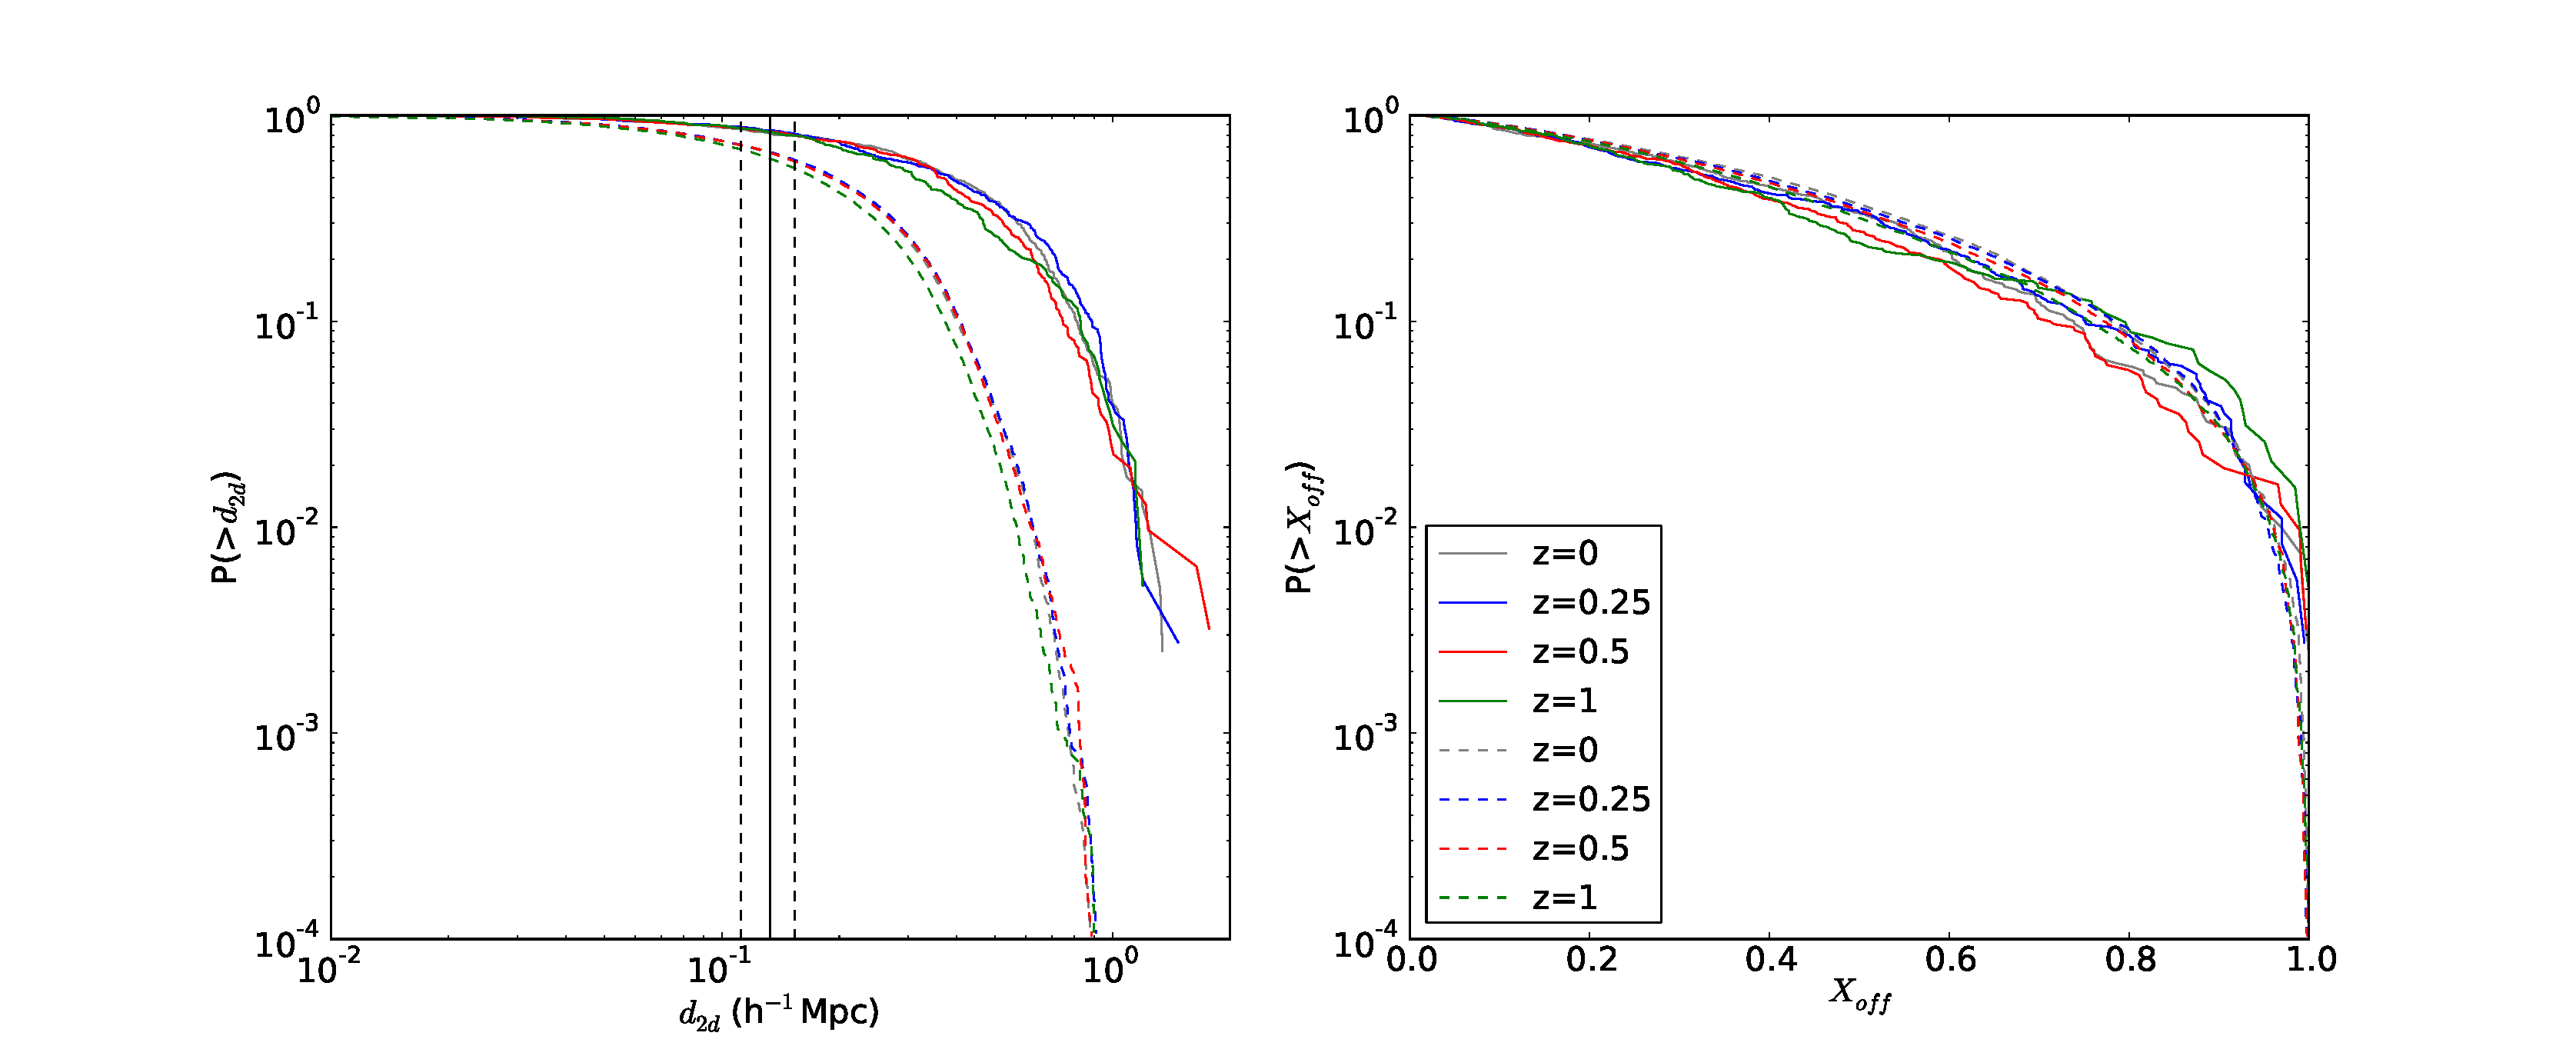
\includegraphics[width=0.8\textwidth]{New_figures/figure_2.eps}
\end{center}
\caption{
  Integrated probability distribution for the displacement
  between the host halo and its dominand sub-halo. The left panel
  shows the results in terms of the physical displacements and the
  right panel the same displacement normalized by the virial radius of
  the host halo. The continous line corrresponds to the halos in the
  group sample $V_{\rm circ,host}>700\kms$ and the dashed lines to the
  sample $V_{\rm circ,host}<700\kms$.
  The vertical stripe corresponds to the estimate of the separation
  between the two dark matter clumps in the results reported by
  \citet{Gastaldello} for the group SL2S J08544-0121. The right panel
  shows the same results normalized by the virial radius of the host
  halo.} 
\label{fig:displacement}
\end{figure*}



\begin{figure*}
\begin{center}
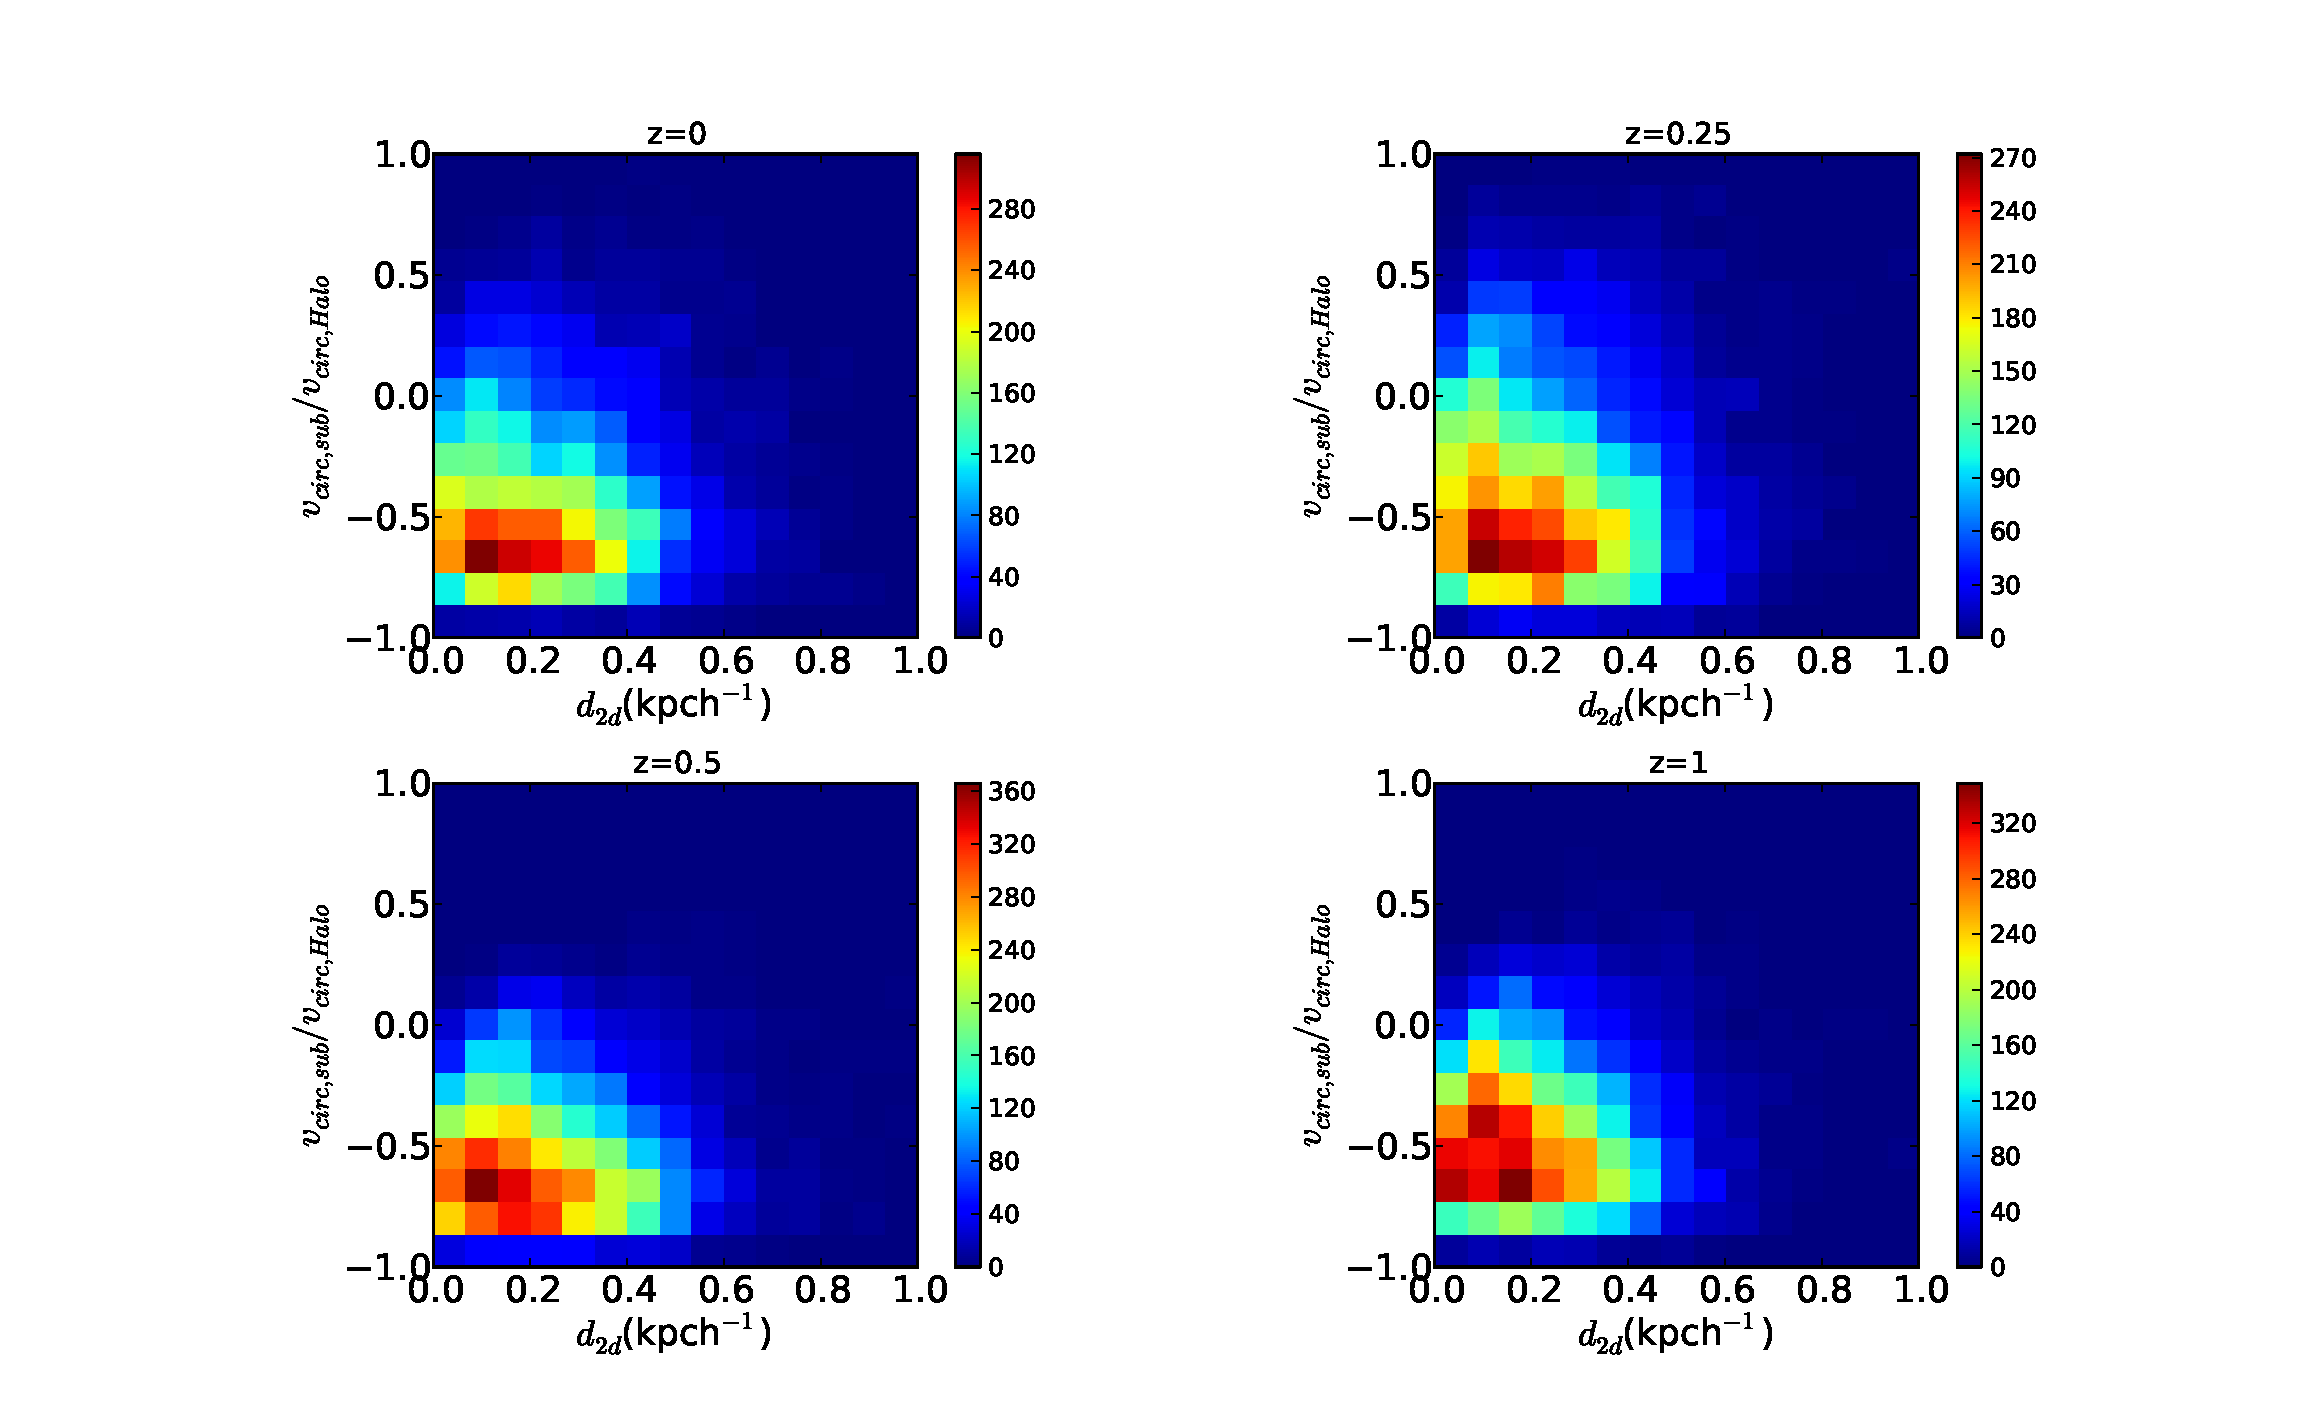
\includegraphics[width=0.8\textwidth]{Figures_eps/figure_4_VcircsubVcirchalo_300kms_700kms.eps}
\end{center}
\caption{2D histogram in the plane $V_{\rm c,sub}/V_{\rm
    c,host}$-$d_{2D}$. The left panel corresponds to groups and the
  right panel to clusters. The circle with error bars corresponds to
  \bullg data reported from \citet{2013A&A...552A..80M} and
  \citet{Gastaldello}. The data used to construct the histograms
  integrates the objects at all redshifts. }
\label{fig:mass_displacement}
\end{figure*}




The main result of this paper is summarized in Figure
\ref{fig:displacement}, it presents the integrated
probability distribution for the displacement between the center of
the host halo and its dominant sub-halo. The left pannel shows
the displacement in physical units and the right pannel as a fraction
of the virial radius of the host halo. 

Figure \ref{fig:displacement} shows the results for two different
populations; groups with $300\kms < V_{\rm c, host}<700\kms$ and
clusters with $V_{\rm c,host}>700\kms$. Additionally, this is
presented for all redshifts $z=0.0, 0.25, 0.5$ and $1.0$. 

The panel with the physical displacements also shows a vertical stripe
with the estimated displacement for the Bullet-group reported by
\cite{Gastaldello}. Considering this system as consistent withe the
groups sample we see that a fraction of $\sim 15\pm 2\%$ of the groups
should present a displacement equal or larger than the one estimated
for \bullg, this fraction is close to $45\pm2\% $. The panel with the
normalized displacements shows a  distribution that can be considered
close to universal in the sense that the two samples (groups and
clusters) at all redshifts present a similar trend.[...]

Figure \ref{fig:mass_displacement} shows 2D histograms in a plane
composed by the ratio of the two circular velocities $V_{\rm c,
  sub}/V_{\rm c, host}$ and the physical displacements. This is
revealing because these two quantities can be constrained by
observations. The displacement is a direct observable, while the ratio
of the circular velocities can be estimated from lensing studies or
approximated by the ratio of the total galaxy luminosity associated
with the galaxy peaks.

To construct this figure we co-add all the halos in the sample (left,
groups; right, clusters) at all redshifts. We stack the data because
we do not observe any strong time evolution, aditionally this allows
us to increase the signal in each bin. Overplotted there is an circle
with error bars that represents the observational estimates for the
system \bullg. 


\subsection{Relative Velocities}
\label{sec:velocities}

\begin{figure}
\begin{center}
\includegraphics[width=0.5\textwidth]{Figures_eps/figure_3.eps}
\end{center}
\caption{Integrated probability distribution for the relative velocity of the
sub-halo with respect to its host. The left panel shows the results
in physical units while the right panel show the same values
normalized by the circular velocity of the host halo. The line coding
follows the same structure as Figure \ref{fig:displacements}}
\label{fig:velocities}
\end{figure}

In Figure \ref{fig:velocities} we present the integrated probability
of the relative peculiar velocities of the sub-halos with respect to
the host halo. The left panel presents this velocity in physical units
while the left panel presents them as a fraction of the circular
velocity of the host halo. 

The panel with the normalized velocities shows that the distribution
of sub-halo velocities is close to universal. Regardless
of the mass of the host halo and the redshift the integrated
distributions lie very close to each other. 

The median of this distribution is located at $v/V_{\rm
  c,host}=1.1$. We also note the strong break at $v/V_{\rm
  c,host}=3.0$ that is present in the data from the group sample that
allows us to probe fractions on the order of $10^{-4}$.  This break is
located close the escape velocity of $v/V_{\rm c,host}$ for dark
matter halos following a NFW profile with a concentration value
$c\approx 6$ \citep{Hayashi2006}. 



\subsection{Collision Geometries}
\label{fig:geometry}

Figure \ref{fig:} presents the geometry of the bullet groups in our 
 the relative geometry of the collision using the
variables $\mu$ and $X_{\rm off}$.

\begin{figure*}
\begin{center}
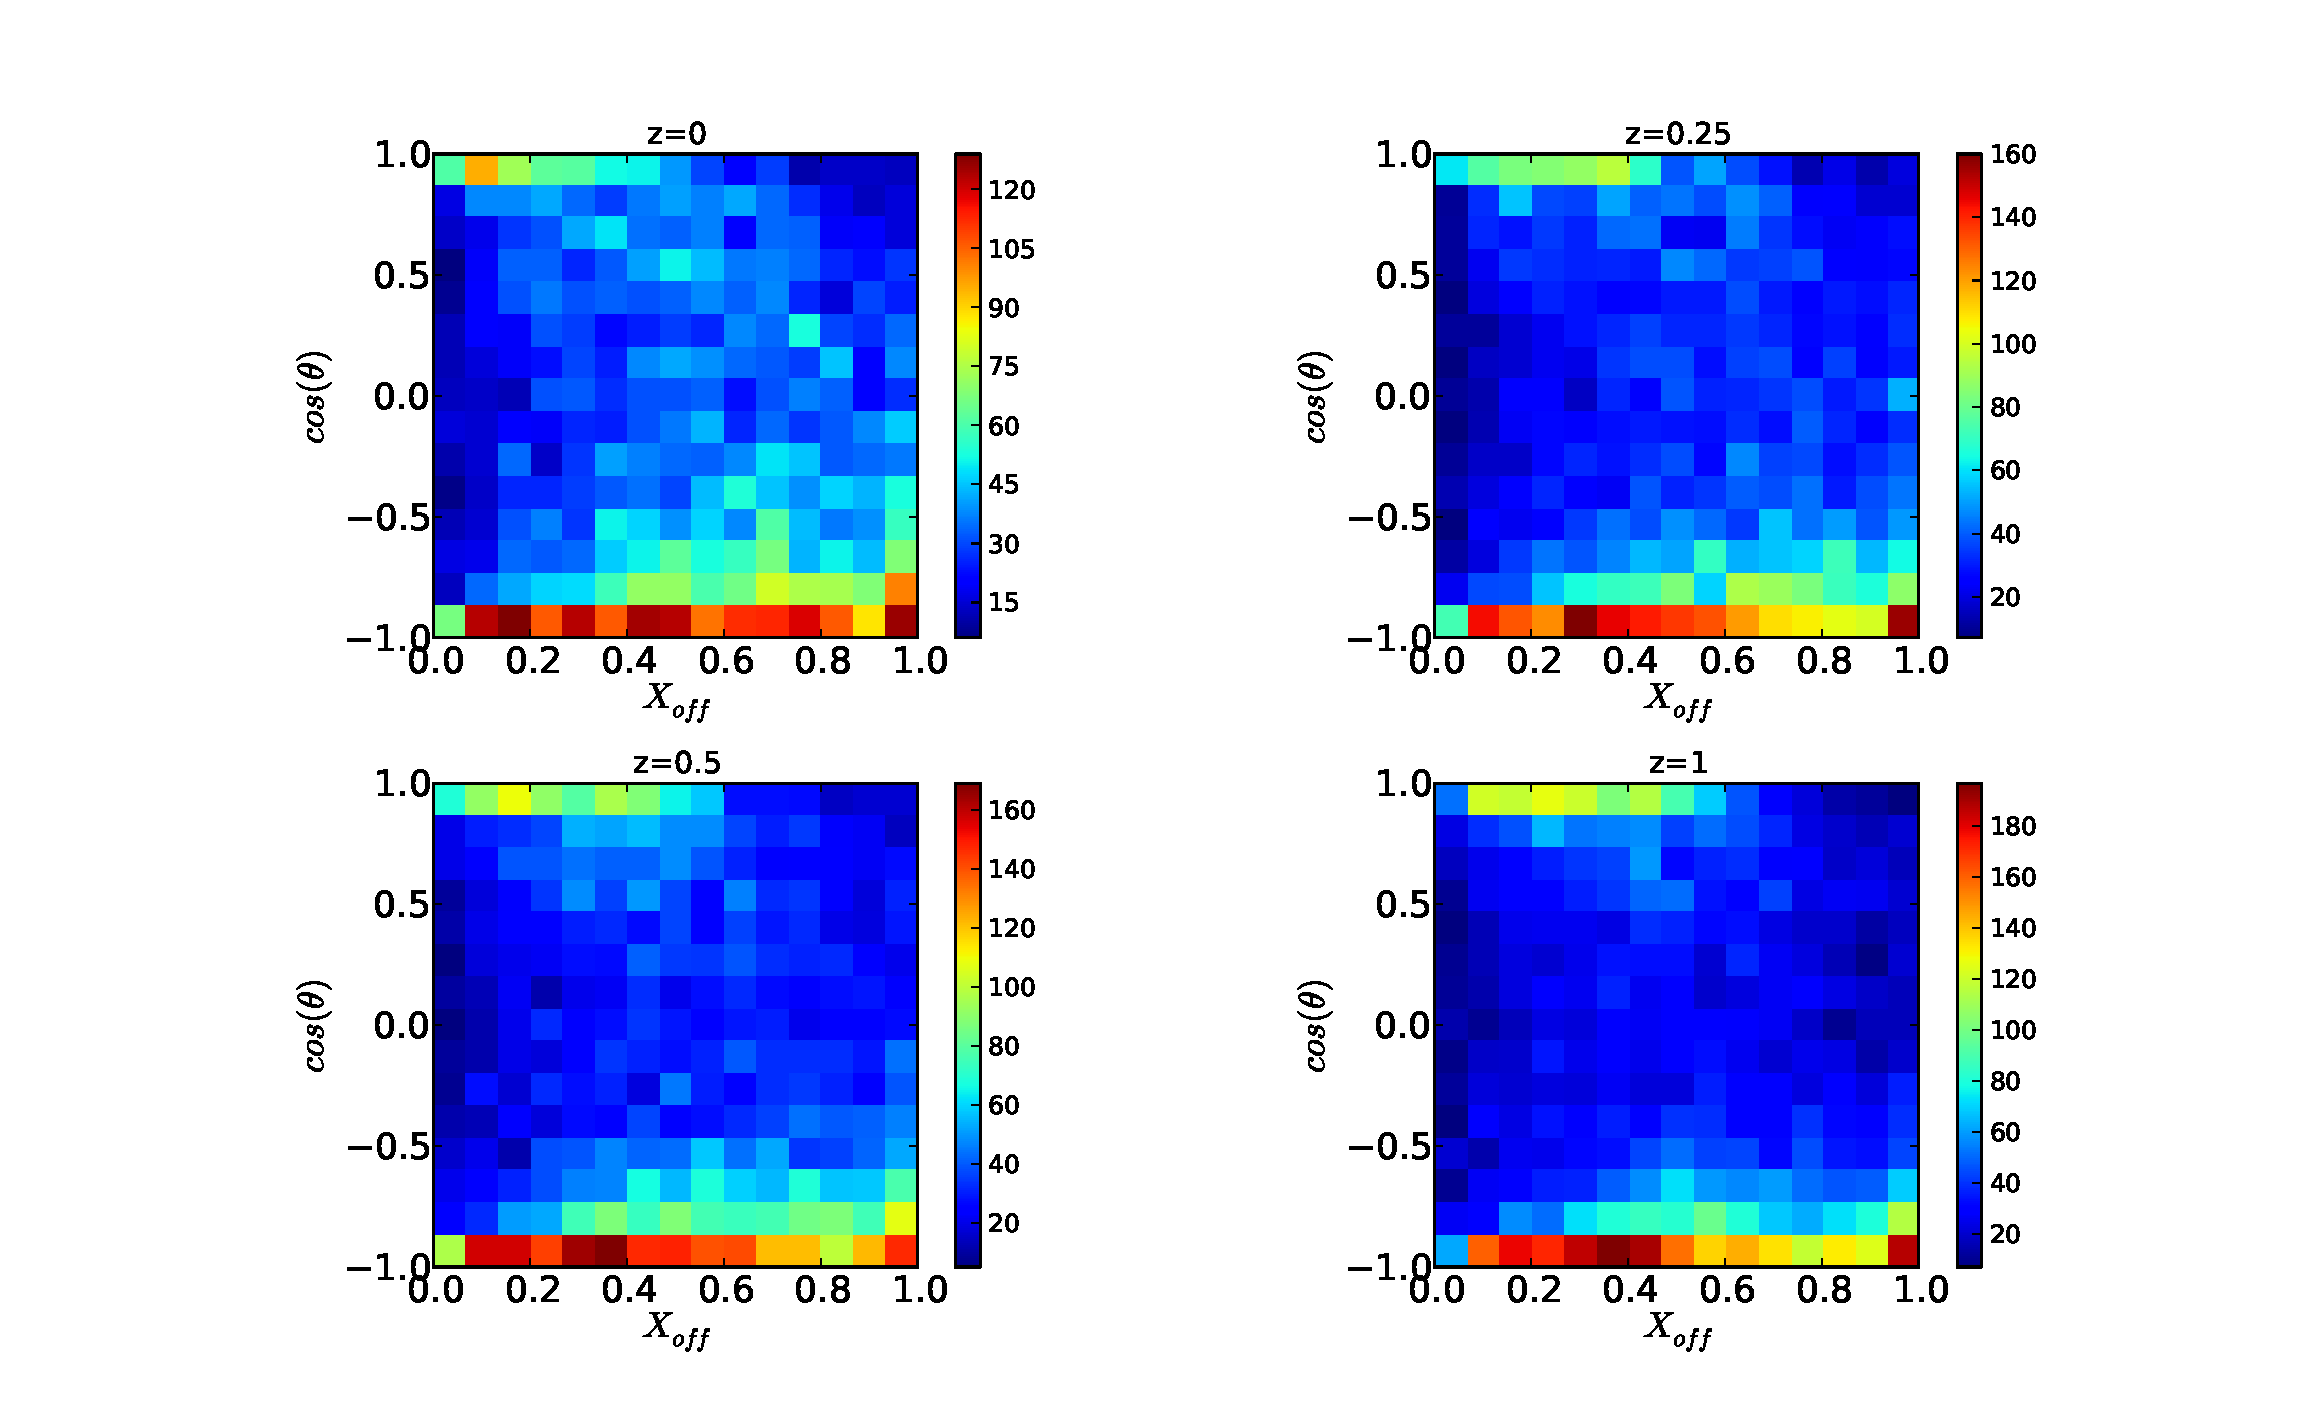
\includegraphics[width=1.0\textwidth]{Figures_eps/figure_4_300kms_700kms.eps}
\end{center}
\caption{x}
\label{fig:geometry}
\end{figure*}


\section{Discussion}
\label{sec:discussion}
Strictly speaking our results apply to multimodal groups and the e
expected separation betwen dark matter clumps. [...]
 
Expected displacement between dark and baryonic components are better
described by systems where the collision already occurred.[...]
(comparison with the old bullet clusters paper?)

The expectations to quantify this effects observationally are
high. [...] 


In order to facilitate the reproducibility and reuse of our results we
have made available all the data and the source code available in a public
repository. [...]  


\section{Conclusions}
\label{sec:conclusions}


We selected four snapshot of the simulation for four different
redshifts (z$=0$, z$=0.25$, z$=0.5$ and z$=1$) based in the
distribution of redshift in the Figure 1 by \citet{verdugo}, and  for
each sample in redshift we selected the host halo with circular
velocities greater than 300 kms$^{-1}$ and was split in two  principal
groups: The first group correspond to host halo with circular
velocities between 300 kms$^{-1}$ to 700 kms${^{-1}}$ with mass in the
range of $10^{12}$ M$_\odot{}$ to $10^{14}$ M$_\odot{}$ in the range
of mass of the Bullet Groups, and second group correspond to host halo
with circular velocities greater than 700 kms$^{-1}$ with mass
$\geq10^{14}$ M$_\odot{}$, in the range of mass of the Bullet
Clusters, in  the Table \ref{table1} is shown the two groups selected
in this work. For each group, we  classified the corresponding
substructures most massive and associated with the corresponding host
halo.  In  this work,
we estimate the expected distribution of displacements
($d_{real,(X,Y)}$) in the projection 2-D that can estimated by
observations, these displacements correspond to the separation between
the minimal potential of the host halo and the  minimal potential of
the substructure, both are dark matter distributions. 



In order to explore the distribution of displacements expected in the observational, we define a new parameter given by:\\

\begin{equation}
 \frac{v_{circ,sub}}{v_{circ,halo}}=0.5
\end{equation}
 

Figure \ref{newparameter} shows the scatter plot of the parameter
$\left(\frac{v_{circ,sub}}{v_{circ,halo}}\right)$ vs the  displacement
($d_{2d,(X,Y)}$) between the host halo and the substructure and for
different redshifts. This parameter is  consistent with the
observations. The red star simbol in the Figure \ref{newparameter} is
equal to 0.54 corresponding to  the fraction in velocity dispersion in
the line-of-sigth of the group SL2S SJ08544-0121
($\sigma_{host,halo}=341^{+43}_{-109}$ kms$^{-1}$ and
$\sigma_{substructure}=185^{+30}_{-62}$), reported by
\citet{2013A&A...552A..80M}. Based in the parameter
$\left(\frac{v_{circ,sub}}{v_{circ,halo}}\right)>0.5$, we estimate the
expected distribution of displacements and this is shown in the Figure
\ref{displacements} for the two groups classified in this work. 
  


 




\section*{Acknowledgements}

The CosmoSim database used in this paper is a service by the
Leibniz-Institute for Astrophysics Potsdam (AIP). The  BolshoiP
simulation was performed within the Bolshoi project of the University
of California High-Performance  AstroComputing Center (UC-HIPACC) and
was run at the NASA Ames Research Center. 


\bibliographystyle{apj}
\bibliography{references} 

\end{document}
